% Geometry, font
\documentclass[12pt, letter]{article}
\usepackage[margin=0.8in]{geometry}
\usepackage[T1]{fontenc}
\usepackage{fourier}
\usepackage{titling}
\setlength{\droptitle}{-5em} 
\usepackage[parfill]{parskip}
\usepackage{graphicx}
\graphicspath{{imgs/}}
\usepackage{hyperref}

% Math stuff
\usepackage{amssymb}
\usepackage{bm}

% Code Highlighting
\usepackage{minted}
\usemintedstyle{solarizedlight}

\author{Zach Neveu}
\title{ Day 8 Notes }

\begin{document}
\maketitle

\section{Agenda}%
\label{sec:agenda}
\begin{itemize}
	\item Matching concepts
	\item Algorithm to solve matching
	\item Bipartite matching
	\item Intro to linear programming
\end{itemize}

\section{Matching Review}%
\label{sec:matching_review}
\begin{itemize}
	\item Review of matching problem from last class
	\item Swapping membership of augmenting path yields larger matching
	\item Maximum matching includes all nodes
	\item Key result: given a matching, M, the matching is optimal if and only if no augmenting path with respect to M exists.
	\item If no augmenting path $\rightarrow$ M is optimal (not so obvious)
	\item If M optimal $\rightarrow$ no augmenting path (this is fairly straightforward)
\end{itemize}
\begin{figure}[h]
    \centering
    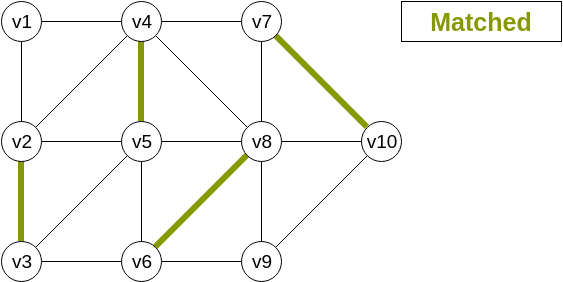
\includegraphics[width=0.6\textwidth]{matching}
    \caption{Review matching diagram from Day 6}
    \label{fig:matching}
\end{figure}

\subsection*{Matching Algorithm}
\begin{minted}{Python}
def match(g):
    m = 0
    while p = aug_path(M):
        swap_membership(p)
\end{minted}

\begin{itemize}
    \item Outer loop runs $O(E)$ times where $E$ is # edges
    \item Time to find an augmenting path is polynomial time
    \item Algorithm to find augmenting path is convoluted and not particularly useful to know
\end{itemize}

\subsection*{Bipartite Matching}
\begin{itemize}
    \item \textbf{Bipartite Graph}: a graph where the nodes can be divided into two groups such that every edge goes from one group to the other (no edges are inside a group).
    \item Bipartite Matching: find the largest matching in a bipartite graph
    \item Classic example problem: Job scheduling on heterogeneous computers
    \begin{itemize}
        \item Group of jobs that all need to be done
        \item Group of computers that can run jobs
        \item Certain jobs can only run on certain computers
        \item Find how to get the most jobs done
    \end{itemize}
\end{itemize}

\begin{figure}[h]
    \centering
    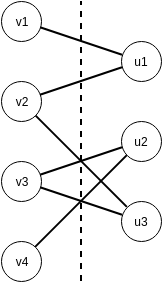
\includegraphics[width=0.2\textwidth]{bipartite}
    \caption{Bipartite Graph Example: Every edge crosses dividing line}
    \label{fig:bipartite}
\end{figure}
\begin{itemize}
    \item Start at all exposed nodes
    \item Do BFS across alternating edges until another exposed node is reached
    \item The path between exposed nodes that is found is an augmenting path
    \item BFS runs in fast polynomial time and fins any augmenting paths that exist
    \item Search diagram has structure: matched stages don't branch, matched and unmatched stages alternate
    \item Why is this like greedy algorithms?
    \begin{itemize}
        \item Matching always getting bigger
        \item Not quite greedy: some edges get deleted when swapping membership
        \item Kind of a ``deeper" greedy algorithm
        \item Approach applicable to many problems
    \end{itemize}
\end{itemize}
\begin{figure}[h]
    \centering
    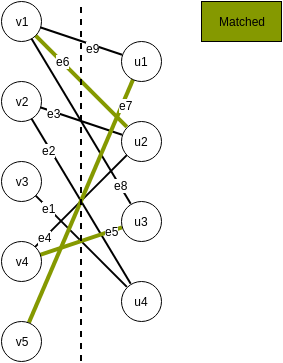
\includegraphics[width=0.4\textwidth]{bipartite-matching}
    \caption{Exaple Bipartite matching}
    \label{fig:bipartite-matching}
\end{figure}

\begin{figure}[h]
    \centering
    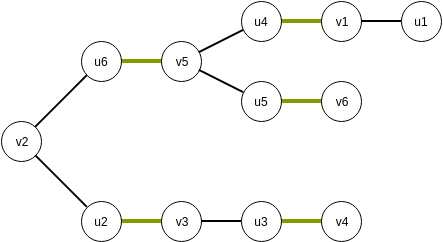
\includegraphics[width=0.5\textwidth]{search-diagram}
    \caption{Example search diagram (different problem from fig. \ref{fig:bipartite-matching})}
    \label{fig:search-diagram}
\end{figure}

\section{Linear Integer Programming (LP)}%
\label{sec:linear_integer_programming}
\begin{itemize}
    \item Many problems have special format
    \item If your problem can be re-phrased into this format, it can be solved FAST by existing solvers.
    \item Leverage genius that is not yours
    \item Not super well known in ECE, came from applied math
    \item Large LP instances solvable in minutes
    \item Trade-off is that problem must be in exact format
\end{itemize}

\subsection*{Example}
\begin{itemize}
    \item You are a politician trying to win an election. Your district has 3 regions:
    \begin{itemize}
        \item Urban - 100k voters
        \item Suburban - 200k voters
        \item Rural - 50k voters
    \end{itemize}
    \item Goal is to get a majority in each region
    \item Win votes by advertising based on 4 issues
    \begin{itemize}
        \item Building roads
        \item Gun control
        \item Farm subsidies
        \item Gas taxes
    \end{itemize}
    \item Goal: get max results within advertising budget
\end{itemize}

\begin{table}[h]
    \centering
    \caption{Problem Breakdown Table}
    \label{tab:label}
    \begin{tabular}{|c|c|c|c|}
    \hline
     & urban & suburban & rural \\
    \hline
    Build roads & 0.2 & 5 & 3 \\
    \hline
    gun control & 8 & 2 & -5 \\
    \hline
    farm subsidies & 0 & 0 & 10 \\
    \hline
    gas taxes & 10 & 0 & -2 \\
    \hline
    \end{tabular}
\end{table}

\end{document}
